Lichtstrahlen werden aufgrund des Brechungsindex gebrochen, wenn sie auf Linsen
\begin{wrapfigure}{l}{6cm}
  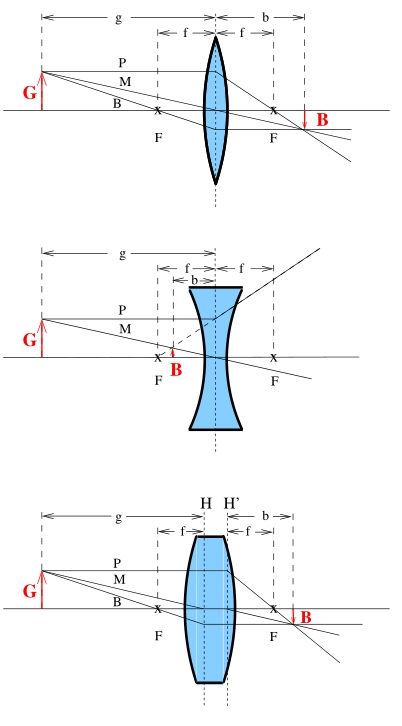
\includegraphics[width=5cm]{bilder/konstruktion.jpg}
  \caption{Bildkontruktion für verschiedene Linsen \cite{408}.}
  \label{fig:kons}
\end{wrapfigure}
treffen. Dies passiert sowohl beim Ein- als auch beim Austreten. Bei den Linsen
lässt sich zwischen Sammel- und Zerstreuungslinse unterscheiden. Je nachdem auf
welche Linse das Licht trifft, wird es anders gebrochen.
Sammellinsen sind doppelseitig konvex und brechen das Licht so, dass parallel
einfallende Strahlen in einem Brennpunkt $\su{B}$ gesammelt werden. Da sowohl die
Brennweite $f$ und die Bildweite positiv sind, wird das entstandene Bild als
reel bezeichnet. Die Zerstreuungslinse hingegen ist doppelseitig konkav und
besitzt eine negative Brenn- und Bildweite. Bilder, die durch Zerstreuungslinsen
entstehen werden als virtuell bezeichnet. Die Bildkonstruktionen für Sammel- und
Zerstreuungslinsen sind in der nebenstehenden Abbildung \ref{fig:kons} dargestellt.
Für die Bildkonstruktion sind drei Strahlen wichtig
\begin{itemize}
  \item Der Parallelstrahl läuft parallel zur optischen Achse vom Objekt zur Linse. Dort wird er gebrochen, sodass er durch den Brennpunkt läuft.
  \item Der Mittelpunktstrahl verläuft vom Objekt zum Mittelpunkt der Linse.
  \item Der Brennpunktstrahl läuft vom Objekt durch den Brennpunkt und zur Linse.
  dort wird er gebrochen und verläuft weiter parallel zur optischen Achse.
\end{itemize}
Das Abbildungsgesetz
\begin{equation}
  V = \frac{B}{G} = \frac{b}{g}
  \label{eqn:abb}
\end{equation}
lässt sich nun mit Hilfe der Strahlensätze an den Beispielen aus Abbildung \ref{fig:kons}
herleiten. Hierbei entspricht $B$ der Bildgröße und $G$ der Objektgröße. Analog
hierzu sind $b$ und $g$ die Bild- beziehungsweise Objektweiten. Die Linsengleichung
lässt sich mit Gleichung \eqref{eqn:abb} und der Bildkonstruktion herleiten und
lautet somit
\begin{equation}
  \frac{1}{f}=\frac{1}{b}+\frac{1}{g}.
  \label{eqn:linse}
\end{equation}
Dass die Brechung an dünnen Linsen nur in an der Mittelebene stattfindet ist eine
Annahme die nur für achsennahe Strahlen zutrifft, da bei achsenfernen Strahlen
Linsenfehler auftreten. Liegt der Brennpunkt der achsenfernen Strahlen näher an
der Linse als der der achsennahen Strahlen lässt sich kein scharfes Bild mehr erzeugen.
Dies wird als sphärische Abberation bezeichnet. Durch Ausblenden der
achsenfernen Strahlen mittels einer Blende lässt sich diese Abbrebation beheben.
Zudem ist der Brechungsindex von der Wellenlänge $\lambda$ des einfallenden Lichts
\begin{wrapfigure}{r}{4cm}
  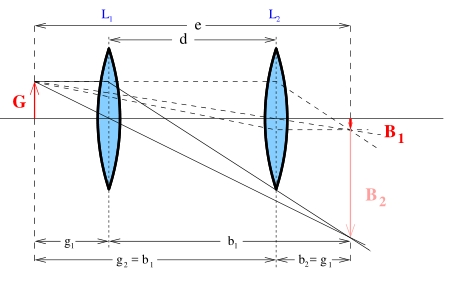
\includegraphics[width=4cm]{bilder/abstande.jpg}
  \caption{Schematische Darstellung der Abstände \cite{408}.}
  \label{fig:abs}
\end{wrapfigure}
abhängig, was chromatische Abberationen zur Folge haben kann.
So wird etwa blaues Licht stärker gebrochen als rotes Licht, da der Brennpunkt
näher an der Linse liegt.

Um die Brennweite $f$ einer Linse zu bestimmen gibt es verschiedene Methoden.
Bei der Methode nach Bessel wird der Abstand $e$ zwischen dem Gegenstand und dem
Schirm konstant gehalten. Hier sollte $e$ mindestens viermal so groß sein wie die
Brennweite $f$ der Linse. Die Linse wird dann zwischen Gegenstand und Schirm
bewegt. Hierbei gibt es zwei Positionen bei denen das Bild scharf auf dem
Schirm abgebildet wird. Da die Linsenpositionen symmetrisch sind gilt
\begin{align*}
  b_1&=g_2, \\
  b_2&=g_1.
\end{align*}
Wie in Abbildung \ref{fig:abs} zu sehen gilt
\begin{align}
  e &= g_1 + b_1 = g_2 + b_2,\\
  d &= g_1 - b_1 = g_2 - b_2.
\end{align}
Aus diesen beiden Formeln lässt sich die Brennweite $f$ dann mit
\begin{equation}
  f = \frac{e^2-d^2}{4e}
\end{equation}
bestimmen.
\begin{wrapfigure}{r}{5cm}
  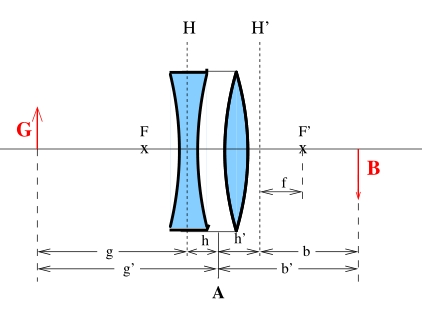
\includegraphics[width=5cm]{bilder/abbe.jpg}
  \caption{Schematische Darstellung der Methode nach Abbe \cite{408}.}
  \label{fig:abbe}
\end{wrapfigure}

Bei der Methode von Abbe wird die Brennweite eines Linsensystems bestimmt. Neben
der Brennweite muss hier auch die Lage der beiden Hauptebenen ermittelt werden
Dazu wird der Abbildungsmaßstab $V$ verwedet. Hierfür werden die Objekt- und die
Bildweiten  $g'$ und $b'$ bezüglich eines beliebigen Punktes $A$ gemessen wie in
Abbildung \ref{fig:abbe} gezeigt. Mit den Formeln
\begin{align}
  \begin{split}
    g' &= g + h = f\,\cdot\,\left(1+\frac{1}{V}\right) + h \\
    b' &= b + h'= f\,\cdot(1+V)+h'
    \label{eqn:haupt}
  \end{split}
\end{align}
lassen sich dann die Hauptebenen $h$ und $h'$ und die Brennweite $f$ bestimmen.
